\section{IEC funksjonsblokker} \label{IEC Seksjon}
\thispagestyle{fancy}

Vi gjorde eit utval av moglege funksjonsblokktemplat basert på dei komponentane vi identifiserte i reinseanlegget.
For å lage eit robust program valde vi å fokusere på to inputfunksjonar, \gls{MA}, \gls{MB}, og to outputfunksjonar \gls{SBE}, \gls{SBV}.
Sjølv om funksjonsblokktemplata kunne verke overkvalifiserte, valde vi likevel inkludere dei, då nokon av tilleggsfunksjonane eventuelt kunne nyttast seinare
og at det gav oss ein klar retning å arbeide mot.

\gls{IEC} har sentrale begrep som vi ønskjer å utdjupe nærmare. Grunna mangel på gode norske begrep
og for å forhindre forvirring velger vi å beskrive begrepa slik dei er skildra i normen. \newline
Merk også forkorting i klammeparantes.

\begin{itemize}
    \item \textbf{Lock:} Action overruling any other signal while being true        \textbf{[L]}
    \item \textbf{Force:} Action overruling any other signal                        \textbf{[F]}
    \item \textbf{Disable transition:} Transistion high/low function not avaliable  \textbf{[D]}
    \item \textbf{Blocking:} Prevention of certain functions or operations          \textbf{[B]}
    \item \textbf{Suppression:} Disable alarm annunciation as well as any associated automatic actions \textbf{[U]}

\end{itemize}

Det er også andre genrelle forkortingar som er viktige i skildring av desse blokkene.

\begin{itemize}
    \item \textbf{X:}   Inngangsvariabel
    \item \textbf{Y:}   Utgangsvariabel
    \item \textbf{B:}   Binær status
    \item \textbf{P:}   Parameter
    \item \textbf{A:}   Alarm handling 
    \item \textbf{W:}   Forvarsel
    \item \textbf{H:}   Høg
    \item \textbf{L:}   Lav
\end{itemize}

For full forståelse av forkortingar og betydning kan ein finne bokstavmatrise i normen.

%Alle funksjonsblokktemplat som er basert på \gls{IEC} \gls{PAS} 63131 har moglegheit for handtering av varsling og feil. 
%Desse funksjonane er viktige i vidare arbeid mot feilhandtering.

\newpage

\subsection{Monitor Binary}
Inputfunksjon \gls{MB} blir brukt til automatisk overvaking, alarmhandtering, framvising og låsing av binære prosessvariablar. \citep{IEC-63131}

\gls{MB} hentar verdi på X og gir tilbake verdi på Y.
Denne utgangsverdien har moglegheit for tidsforseinking, invertering og 

Funksjonsblokka inkluderer alarm ``suppression'' og ``blocking'' funksjonalitet. Den har moglegheit for invertering av 
inngangssignal og moglegheit for tidsforseinking av utgangssignal via parameter. (Vedlegg C.1)

Funksjonsblokka er brukt i programmet for å overvake alle digitale inngangar t.d. pressostat og nivåvipper.


\begin{figure}[htbp]
    \centering
    \begin{subfigure}[b]{0.45\textwidth}
        \centering
        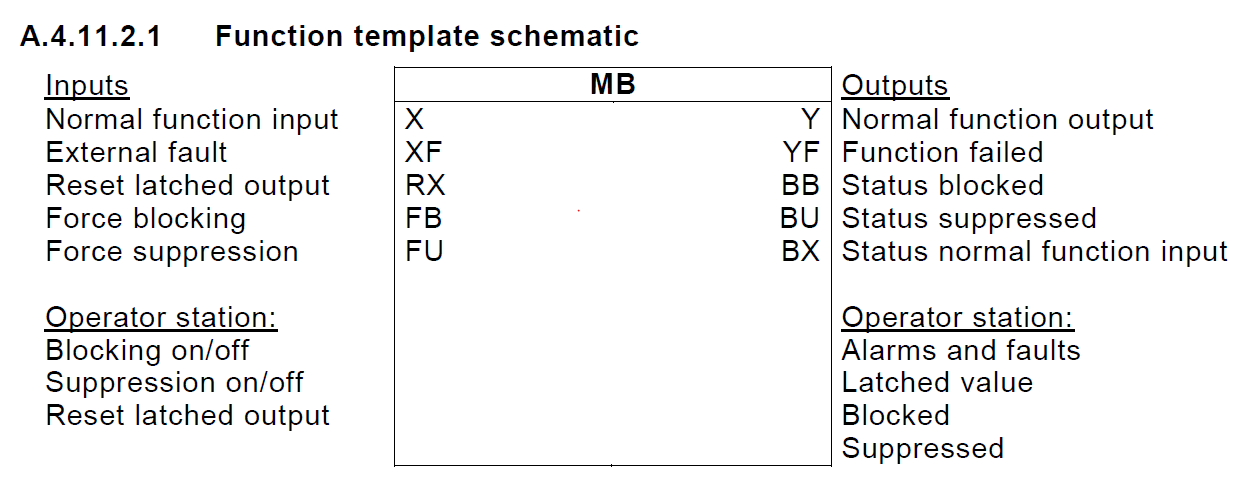
\includegraphics[width=1\textwidth]{Bilder/MBBlokkIEC.png}
        \caption{IEC}\label{fig:Monitor Binary blokk IEC}
    \end{subfigure}
    \hfill
    \begin{subfigure}[b]{0.45\textwidth}
        \centering
        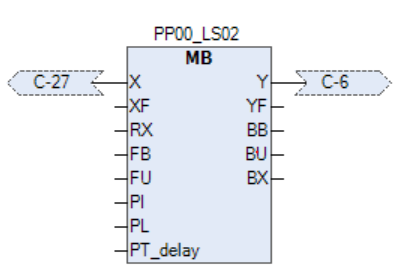
\includegraphics[width=0.7\textwidth]{Bilder/MBBlokkIProgrammet.png}
        \caption{Bruk i programmet}\label{fig:Monitor Binary blokk i programmet}
    \end{subfigure}
    \caption{Monitor Binary}\label{fig:Monitor Binary}
\end{figure}

\newpage

\subsection{Monitor Analogue}
Inputfunksjon \gls{MA} er brukt for skalering, visning, overvaking og alarmhandtering av
analoge prosess og kontrollvariablar \citep{IEC-63131}
Funksjonsblokka er brukt for å overvake analoge trykknivågivarar 
og å skalere og vise desse som ein fyllingsgrad i prosent. (Vedlegg C.2)

\gls{MA} hentar rå verdi på X og gir tilbake verdi på Y.
Denne utgangsverdien blir skalert basert på parameter og har hysterese og dødband tilgjengeleg.

Funksjonsblokka har to forvarsel (WH og WL) og to handlingar med alarm (AHH og ALL).
Det er moglegheit for tidsforsinking, ``blocking'' og ``suppression'' av desse via inngangsvariablar og parameter.

Blokka har fem statusvariablar som indikerer modus og område (BU, BB, BHH, BLL, BBLL, BBHH), ein utgang for indikasjon av feil (YF)
og fire hendingar (BXHH, BXH, BXLL, BXL) utan ``blocking'' og ``suppression'' som nyttast for styring.

Grenser på varsling og hendigar er justerbare via parameter.

\begin{figure}[htbp]
    \centering
    \begin{subfigure}[b]{0.45\textwidth}
        \centering
        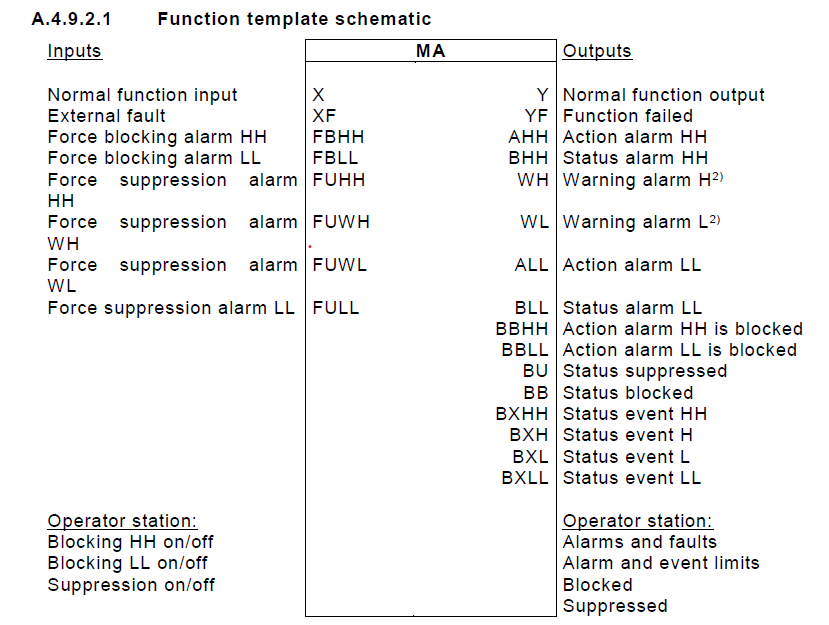
\includegraphics[width=1\textwidth]{Bilder/MABlokkIEC.png}
        \caption{IEC}\label{fig:Monitor Analogue blokk IEC}
    \end{subfigure}
    \hfill
    \begin{subfigure}[b]{0.45\textwidth}
        \centering
        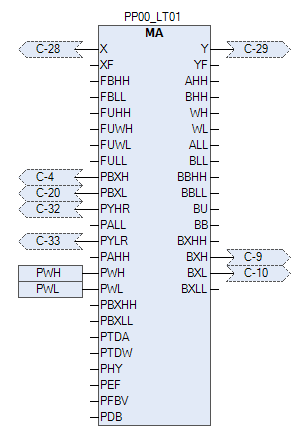
\includegraphics[width=0.7\textwidth]{Bilder/MABlokkIProgrammet.png}
        \caption{Bruk i programmet}\label{fig:Monitor Analogue blokk i programmet}
    \end{subfigure}
    \caption{Monitor Analogue}\label{fig:Monitor Analogue}
\end{figure}

\newpage

\subsection{Switch Binary Eletrical} 

\gls{SBE} funksjonsblokka (Vedlegg C.3) blir brukt for binærkontroll (av/på) av straumningselement for elektrisitet, varme eller væske. 
Den kontrollerte komponenten kan vere t.d. motor, pumpe, varmeelement, vifte.
Funksjonsblokka er i dette programmet brukt til å styre motorar, pumper og blåserar.

%Funksjonsblokka beskriver korleis ein styrer ein komponent.
%Det er utgangen Y, som sender ein opne/stenge kommando (høg/lav) til komponenten. 

%Blokka har fleire funksjonar t.d. samalikning med tilbakemelding \gls{XGH} som gjer korrekt \gls{BCL}/\gls{BCH} status. 

Funksjonsblokka inkluderar alarm ``suppression'', ``blocking'', ``safeguarding'' og ``transition'' funksjonalitet.

\begin{figure}[htbp]
    \centering
    \begin{subfigure}[b]{0.45\textwidth}
        \centering
        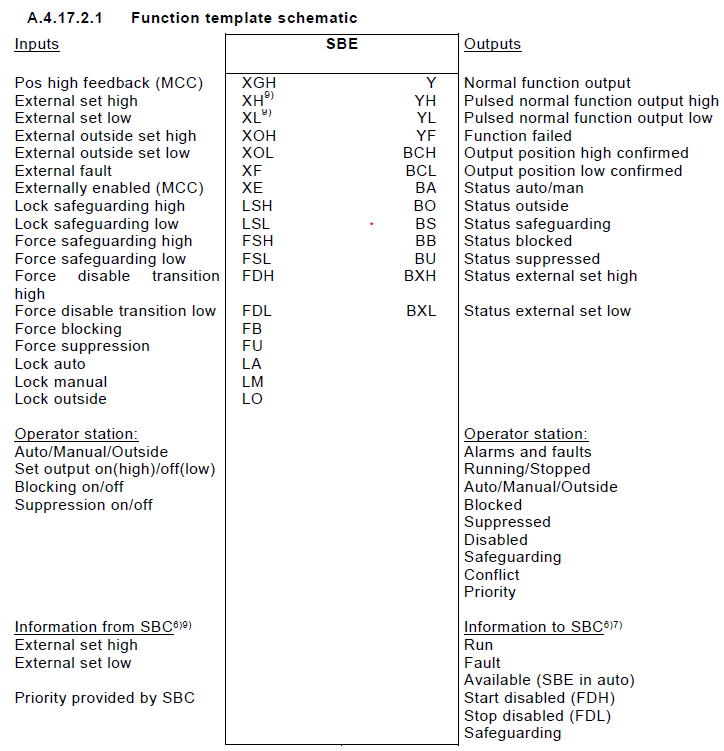
\includegraphics[width=1\textwidth]{Bilder/SBEBlokkIEC.png}
        \caption{IEC}\label{fig:Switch Binary Eletrical blokk IEC}
    \end{subfigure}
    \hfill
    \begin{subfigure}[b]{0.45\textwidth}
        \centering
        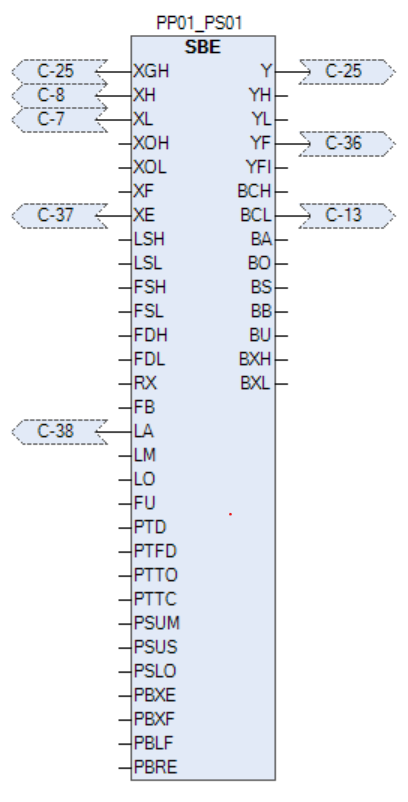
\includegraphics[width=0.5\textwidth]{Bilder/SBEBlokkIProgrammet.png}
        \caption{Bruk i programmet}\label{fig:Switch Binary Eletrical blokk i programmet}
    \end{subfigure}
    \caption{Switch Binary Eletrical}\label{fig:Switch Binary Eletrical}
\end{figure}

\newpage

\subsection{Switch Binary Valve}

\gls{SBV} funksjonsblokka (Vedlegg C.4) skal brukast til binær av/på kontroll av eit straumningselement ved å endra straumen av medium (varme eller væske). 
Typisk komponentar som styrast er bl.a.\ ventilar og spjeld.
Funksjonsblokka er i dette programmet brukt til å styre ventilar.

%Funksjonsblokka styrer ventilen ved hjelp av dei binære inngangane \gls{XH} og \gls{XL}.\@
%Desse inngangane styrer ein utgang Y, som sender opne/stenge-kommando (høg/låg) til ventilaktivatoren.
%Alternativt kan dei pulsmodulerte utgangane \gls{YH} og \gls{YL} kan også nyttast.

Funksjonsblokka har også inngangar \gls{XGH} og \gls{XGL} som gjer tilbakemelding om ventilen er heilt open eller stengd
%som bekrefter ventilen sin posisjon.

Funksjonsblokka inkluderar alarm ``suppression'', ``blocking'', ``safeguarding'' og ``transition'' funksjonalitet.

\begin{figure}[htbp]
    \centering
    \begin{subfigure}[b]{0.45\textwidth}
        \centering
        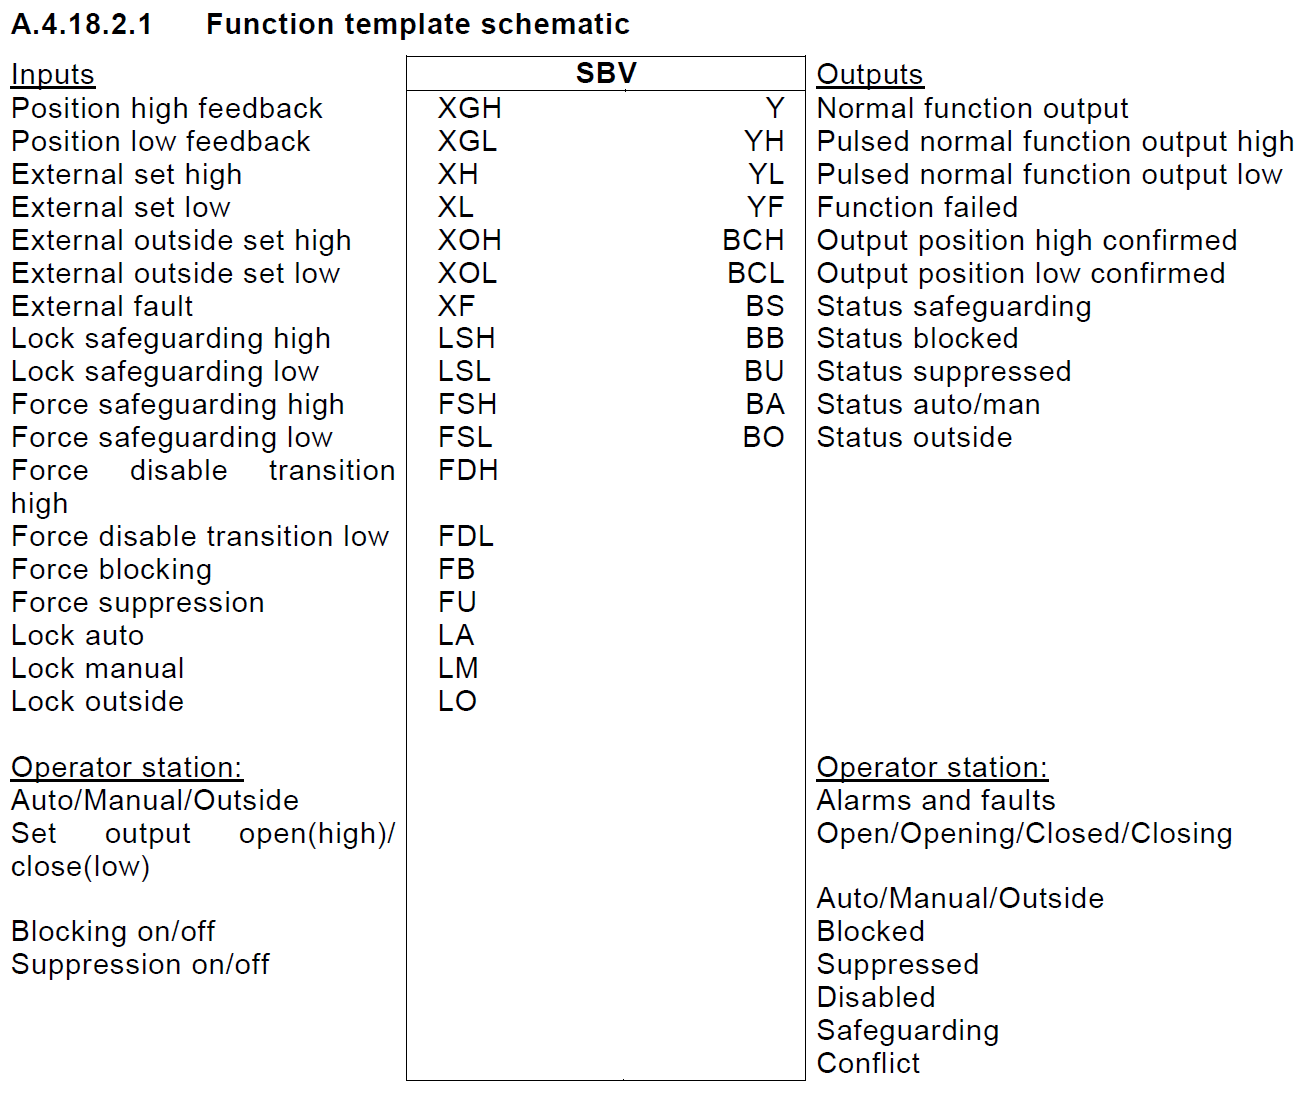
\includegraphics[width=1\textwidth]{Bilder/SBVBlokkIEC.png}
        \caption{IEC}\label{fig:Switch Binary Value blokk IEC}
    \end{subfigure}
    \hfill
    \begin{subfigure}[b]{0.45\textwidth}
        \centering
        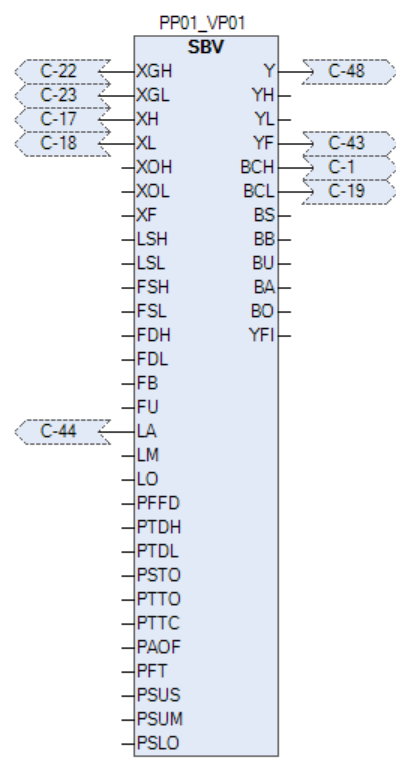
\includegraphics[width=0.5\textwidth]{Bilder/SBVBlokkIProgrammet.png}
        \caption{Bruk i programmet}\label{fig:Switch Binary Value blokk i programmet}
    \end{subfigure}
    \caption{Switch Binary Value}\label{fig:Switch Binary Value}
\end{figure}

\newpage



\newpage

%\begin{figure}[htbp]
%    \centering
%    \begin{subfigure}[b]{0.45\textwidth}
%        \centering
%        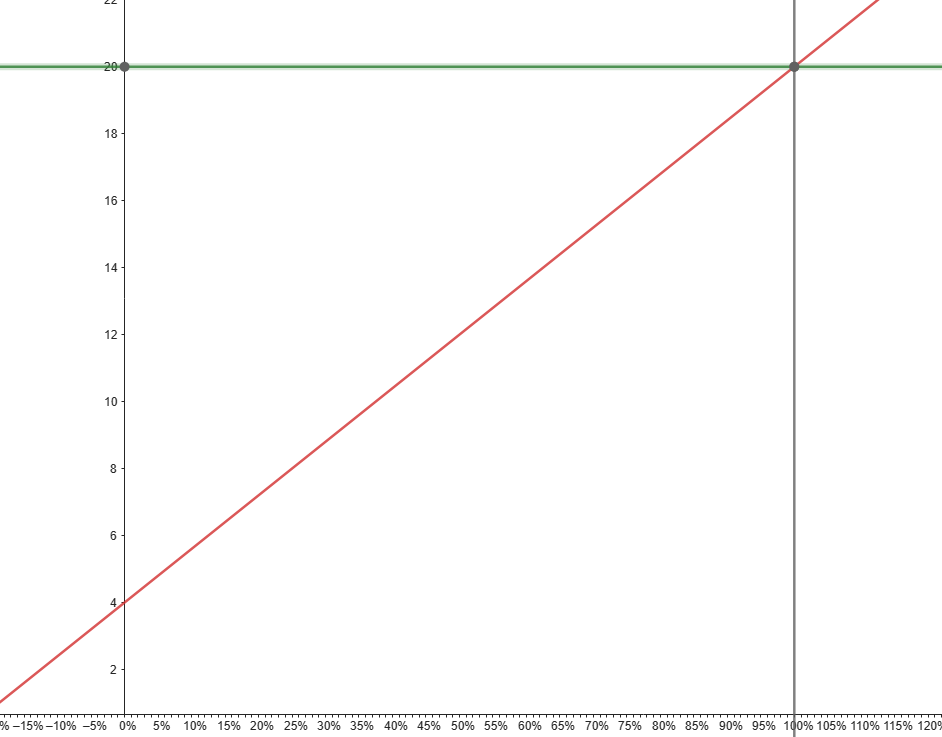
\includegraphics[width=1\textwidth]{Bilder/4_20mA_Scaling.png}
%        \caption{Skalering av mA mot prosent}\label{fig:Skalering av mA mot prosent}
%    \end{subfigure}
%    \hfill
%    \begin{subfigure}[b]{0.45\textwidth}
%        \centering
%        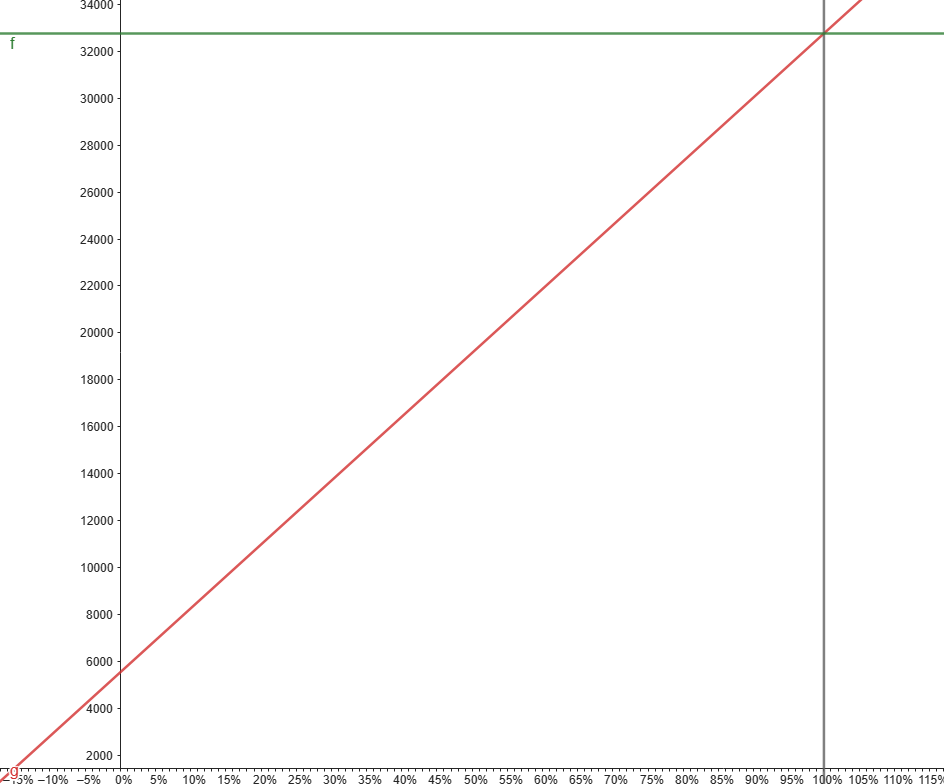
\includegraphics[width=0.95\textwidth]{Bilder/27327_prosent_Scaling.png}
%        \caption{Skalering av prosent til verdi}\label{fig:Skalering av prosent til verdi}
%    \end{subfigure}
%    \caption{Dei forskjellige skaleringane av inngangssignal}\label{fig:Skalering av prosent til verdi}
%\end{figure}


